\documentclass[11pt,a4paper,twoside]{tesis}
% SI NO PENSAS IMPRIMIRLO EN FORMATO LIBRO PODES USAR
%\documentclass[11pt,a4paper]{tesis}

\usepackage{graphicx}
\usepackage[utf8]{inputenc}
\usepackage[spanish]{babel}
\usepackage[left=3cm,right=3cm,bottom=3.5cm,top=3.5cm]{geometry}
\usepackage[version=3]{mhchem}	%fórmulas químicas
\usepackage{siunitx}			%unidades
\usepackage{verbatim}
\usepackage{caption}
\usepackage{subcaption}

%Definiciones de unidades y fórmulas químicas
\sisetup{per-mode = symbol}
\newcommand{\h}{\ce{H^+}}
\newcommand{\oh}{\ce{OH^-}}
\newcommand{\na}{\ce{Na^+}}
\newcommand{\cl}{\ce{Cl^-}}
\newcommand{\nm}{ \si{\nano\metre} }
\newcommand{\um}{ \si{\micro\metre} }
\newcommand{\usec}{ \si{\micro\second} }
\newcommand{\vcm}{ \si{\volt\per\centi\metre} }
\newcommand{\kvm}{ \si{\kilo\volt\per\metre} }
\newcommand{\kvcm}{ \si{\kilo\volt\per\centi\metre} }
\newcommand{\ms}{ \si{\milli\second} }

\begin{document}

\graphicspath{
	{graficos/}
}

% Carátula
\def\titulo{Licenciado }

\def\autor{Mauricio Alfonso}
\def\tituloTesis{Estudio de los Mecanismos Básicos de Electroporación a Través de la Modelación Numérica}
\def\runtitulo{Estudio de los Mecanismos Básicos de Electroporación a Través de la Modelación Numérica}
\def\runtitle{Study of the Basic Mechanisms of Electroporation Through Numeric Modelling}
\def\director{Alejandro Soba}
\def\codirector{Guillermo Marshall}
\def\lugar{Buenos Aires, 2014}
\newcommand{\HRule}{\rule{\linewidth}{0.2mm}}
%
\thispagestyle{empty}

\begin{center}\leavevmode

\vspace{-2cm}

\begin{tabular}{l}

\includegraphics[width=2.6cm]{logofcen.pdf}
\end{tabular}


{\large \sc Universidad de Buenos Aires

Facultad de Ciencias Exactas y Naturales

Departamento de Computaci\'on}

\vspace{6.0cm}

%\vspace{3.0cm}
%{
%\Large \color{red}
%\begin{tabular}{|p{2cm}cp{2cm}|}
%\hline
%& Pre-Final Version: \today &\\
%\hline
%\end{tabular}
%}
%\vspace{2.5cm}

{\huge\bf \tituloTesis}

\vspace{2cm}

{\large Tesis presentada para optar al t\'{\i}tulo de\\
\titulo en Ciencias de la Computaci\'on}

\vspace{2cm}

{\Large \autor}

\end{center}

\vfill

{\large

{Director: \director}

\vspace{.2cm}

{Codirector: \codirector}

\vspace{.2cm}

\lugar
}

\newpage\thispagestyle{empty}


%Abstracts, etc
\frontmatter
\pagestyle{empty}
%\begin{center}
%\large \bf \runtitulo
%\end{center}
%\vspace{1cm}
\chapter*{\runtitulo}

\noindent 

Esto hay que reescribirlo todo! La electroporación reversible es un método consistente en la aplicación de pulsos eléctricos de alta intensidad a una célula con el objetivo de permeabilizar su membrana creando poros, y así permitir el ingreso de drogas o moléculas de ADN a su interior. Esto permite tratar tumores con menores cantidades de drogas, reduciendo los efectos secundarios. En este trabajo se simula una célula esférica a la que se le aplica un pulso eléctrico de 20\si{\milli\second} de duración a través de dos electrodos, y se estudia el ingreso al interior de la célula de 4 especies iónicas: el ión hidrógeno (\h), el hidróxido (\oh), el catión sodio (\na) y el cloruro (\cl). Para eso se tiene en cuenta el campo eléctrico producido por los electrodos, la generación y evolución de poros en la membrana celular producto de la diferencia de potencial entre el interior y exterior de la célula , y la migración de las especies mencionadas, producto de la diferencia de potencial.
Las simulaciones se realizaron con el método de elementos finitos sobre mallas bidimensionales que representan el dominio sobre un sistema de coordenadas cilíndricas usando elementos cuadrilaterales.

\bigskip

\noindent\textbf{Palabras claves:} Guerra, Rebelión, Wookie, Jedi, Fuerza, Imperio (no menos de 5).

\cleardoublepage
%\begin{center}
%\large \bf \runtitle
%\end{center}
%\vspace{1cm}
\chapter*{\runtitle}

\noindent 
%La electroporación consiste en la aplicación de pulsos eléctricos de alta intensidad y corta duración con el objetivo de crear poros en la membrana celular, logrando así un aumento de la permeabilización que permite el ingreso de drogas o iones a su interior. 
Electroporation involves the application of electric pulses of high intensity and short duration in order to create pores in the cell membrane, thus achieving increased permeabilization that allows the entry of drugs or ions.
%La utilización de la electroporación en combinación con drogas antitumorales ha demostrado tener una significativa mayor eficacia que la terapia quimioterapéutica convencional, de allí la relevancia de estudios básicos de la interacción campos eléctricos-célula. 
The use of electroporation in combination with antitumor drugs has been shown to have a higher efficiency than conventional chemotherapeutic therapy, hence the relevance of basic studies of the electric field-cell interaction.
%En esta tesis se presenta un nuevo modelo numérico que describe la respuesta eléctrica de la célula, en particular la membrana celular y el transporte iónico a través de la misma, a la aplicación de pulsos eléctricos. 
In this thesis a new numerical model is presented, describing the electrical response of the cell, particularly the cell membrane and ion transport through it, to the application of electrical pulses.
%Se asume una célula esférica sometida a pulsos eléctricos por medio de dos electrodos, constituida por cuatro especies iónicas: el ión hidrógeno (\h), el hidróxido (\oh), el catión sodio (\na) y el cloruro (\cl). 
A spherical cell is assumed, subjected to electrical pulses by means of two electrodes and consisting of four ionic species: hydrogen ion (\h), hydroxide (\oh), sodium cation (\na) and chloride (\cl).
%Para resolver las ecuaciones diferenciales que describen el potencial electrostático y el transporte iónico se usó el método de los elementos finitos en dos dimensiones espaciales en coordenadas cilíndricas. 
To solve the differential equations describing the electrostatic potential and ion transport, the finite element method in two spatial dimensions with cylindrical coordinates is used.
%Las ecuaciones diferenciales que describen la evolución de la población de poros se resuelven por diferencias finitas utilizando el método de Euler. 
The differential equations describing the evolution of the population of pores are solved by finite differences using Euler's method.
%Se utilizó programación distribuida basada en OpenMP para aprovechar al máximo los procesadores multithreading actuales. 
Distributed programming based on OpenMP was used to maximize the usage of current multithreading processors.
%El nuevo modelo teórico introducido permite por primera vez predecir realísticamente la respuesta eléctrica de la célula, en particular el campo eléctrico transmembranal y el transporte iónico (uptake), lo que se evidencia por la excelente correlación entre predicción y mediciones.
The new theoretical model presented realistically predicts for the first time the electrical response of the cell, particularly the electric field and ion transport (uptake), as evidenced by the excellent correlation between predictions and measurements. 

\bigskip

\noindent\textbf{Keywords:} cell membrane, electroporation, transport, finite elements

\cleardoublepage
\tableofcontents

\mainmatter
\pagestyle{headings}

%Contenido de la tesis

%TODO revisar Underful \hbox warnings
%TODO Comparar tamaños con texmaker
%TODO estilo carátula

% Si tarda mucho en compilar se puede poner cada capítulo en archivos separados.

% CAP 1 introducción. problemática e introducción del modelo
% CAP 2 descripción del modelo. qué se resuelve, método numérico. Explicación de FEM
% CAP 3 ITV. como se resuelve, resultados (solos, sin poros ni transporte)
% CAP 4 Poros. ecuaciones, como se resuelve, resultados
% CAP 5 Transporte. idem (solo transporte, sin poros)
% CAP 6 Todo acoplado. Resultados. poner snapshots de valores 1-9
% CAP 7 conclusiones

\chapter{Introducción}
% CAP 1 introducción. problemática e introducción del modelo

%TODO sacar todos los newline innecesarios (ver otras tesis)

El proceso de electroporación celular tiene como objetivo permeabilizar la membrana de una célula, mediante la aplicación de un campo electromagnético externo, para lograr el transporte a través de la misma de drogas o agentes terapéuticos cargados por difusión y convección. Este proceso es utilizado en diferentes tratamientos electroquímicos de tumores [1,2] como por ejemplo, en la electroquimioterapia (ECT) donde se utilizan drogas quimioterápicas clásicas o en el caso de la Electroterapia Génica (GET), en donde se utilizan moléculas de ADN y ARN[4]. El proceso se optimiza cuando ese campo es pulsado, dependiendo del voltaje aplicado, la duración de los pulsos y la frecuencia de los mismos [3,4].\\

La membrana está compuesta por una bicapa lipídica con su interior hidrofóbico, que actúa como una barrera altamente impermeable a la mayoría de moléculas polares, impidiendo que la mayor parte del contenido hidrosoluble de la célula salga de ella. \\

A tiempo infinito  cualquier molécula difundirá a través de una bicapa lipídica libre de proteínas, a favor de su gradiente de concentración. Sin embargo la velocidad a la que una molécula difunde a través de una bicapa lipídica varía enormemente, dependiendo en gran parte del tamaño de la molécula y de su solubilidad relativa al aceite (es decir, cuanto más hidrofóbica o no polar), tanto más rápidamente difundirá a través de una bicapa [12]. Una de las funciones mas importantes de la membrana es controlar la comunicación entre el medio intracelular y el exterior a través del transporte. Dentro de la célula tienen lugar dos tipos de transporte que se llevan a cabo a través de la membrana: el transporte pasivo y el activo. \\

El transporte pasivo consiste en un proceso de difusión de sustancias a través de la membrana dado por la diferencia de concentración de las mismas. Estos procesos son naturales y no requieren de energía externa. El transporte activo, en cambio, es un proceso que necesita de energía para transportar las moléculas de uno a otro lado de la membrana a través de una permeabilización natural o artificial de la misma.\\

La electroporación de la membrana se inicia con la aplicación de un campo eléctrico que sobre la célula genera el llamado potencial transmembranal (PTM), una diferencia de voltaje inducida sobre la membrana celular que aísla a la célula del medio exterior [5] debido a que la conductividad eléctrica de la membrana es seis (6) órdenes de magnitud más pequeña que la de los medios intra y extra celular. Este potencial inducido tiene estrecha relación con la formación de poros acuosos que conducen a través de la membrana que poseen una dinámica relacionada con el PTM [8]. Sin potencial aplicado dichos poros poseen un radio relativamente pequeño, (del orden de medio nanómetro) que sólo permiten el paso de sustancia específicas de un medio al otro producto de reacciones electroquímicas en su proximidad. La mayor o menor facilidad de las moléculas para atravesar la membrana celular dependen de la carga eléctrica y la masa molar. Moléculas pequeñas o con carga eléctrica neutra pasan la membrana más fácilmente que elementos cargados eléctricamente y moléculas grandes. Además, la membrana es selectiva, lo que significa que permite la entrada de unas moléculas y restringe la de otras.\\
Las moléculas pequeñas no polares se disuelven fácilmente en las bicapas lipídicas y por lo tanto difunden con rapidez a través de ellas. Las moléculas polares sin carga si su tamaño es suficientemente reducido también difunden rápidamente a través de una bicapa. Ejemplos de estas sustancias no polares son los solventes orgánicos, que presentan una polaridad alta o baja. Por ejemplo: el metanol, la acetona, el etanol, la urea, etc.\\

La permeabilidad depende de los siguientes factores: i) Solubilidad en los lípidos: Las sustancias que se disuelven en los lípidos (moléculas hidrófobas, no polares) penetran con facilidad en la membrana dado que está compuesta en su mayor parte por fosfolípidos. ii) Tamaño: la más grande parte de las moléculas de gran tamaño no pasan a través de la membrana. Solo un pequeño número de moléculas polares de pequeño tamaño pueden atravesar la capa de fosfolípidos. iii) Carga: Las moléculas cargadas y los iones no pueden pasar, en condiciones normales, a través de la membrana. Sin embargo, algunas sustancias cargadas pueden pasar por los canales proteicos o con la ayuda de una proteína transportadora.\\

Sin embargo cuando se aplica un campo eléctrico al medio, la población de poros de la membrana responden al PTM en forma dinámica, abriéndose a medida que este potencial aumenta, para después cerrarse en muchos casos o alcanzar un tamaño estable en otros siguiendo una compleja estadística analizada en [7]. En respuesta a esta apertura se modifica el coeficiente de conductividad eléctrica y el de difusión de la membrana facilitando el transporte a través de la misma [6]. Básicamente en este caso por mecanismos guiados por la difusión y la movilidad de las especies iónicas. Estos fenómenos también se relacionan con la tension elástica sobre la membrana. Una campo eléctrico aplicado sobre la misma genera mediante el tensor de Maxwell una tension local que produce una deformación en la célula, que genera que la misma tome una forma oblada o prolada, según sean los campos aplicados [13-14]. Una vez abiertos los poros y deformada la membrana en la zona de los polos de la célula, se produce una condición adecuada para que las especies iónicas de concentración distinta en cada medio (intra y extra celular) comiencen a ingresar dentro de la célula por diferencia de concentración. \\

Es necesario destacar que el modelo propuesto en esta tesis y que sigue el trabajo de diferentes autores [8-12] es un mecanismo aun no establecido con firmeza y sobre el que persisten algunos puntos que aun se deben analizar y continuar estudiando. Es por ese motivo que investigaciones de este tipo resultan valiosas ya que permiten confirmar predicciones y poner en duda suposiciones analíticas que no son tenidas en cuenta por las teóricas y deben ser estudiadas en detalle. \\

Este conjunto de simulaciones deben encararse mediante una compleja batería de modelos acoplados unos con otros y mutuamente dependientes. En esta tesis se propone por primera vez un mecanismo de funcionamiento en conjunto de todos estos fenómenos. Cada uno de estos modelos debe ser abordado por una técnica numérica adecuada. En primer lugar nos proponemos simular la distribución de potencial y campo eléctrico sobre el dominio conformado por el líquido intracelular, el liquido extracelular y la membrana mediante el método de los elementos finitos [9-10], discretizando explícitamente la membrana celular [8,9]. Es necesario destacar que la membrana celular posee un espesor aproximado de entre 5 y 10 nanómetros representando un desafío numérico novedoso al intentar discretizar la misma mediante elementos finitos. En la literatura la membrana es tratada mediante una condición de contorno que separa los medios extra e intra celular [12]. \\

La modelización de la dinámica de creación y evolución de la población de poros sobre la membrana y el tamaño de los mismos es resuelta medianate una serie de ecuaciones diferenciales ordinarias, que se evolucionan en el tiempo mediante un algoritmo de un paso usual [15]. Con la información provista por ambos modelos, calculamos la nueva conductividad eléctrica y el coeficiente de difusión de la membrana permeabilizada, así como la distribución de tensiones sobre la misma. Tensión que retroalimenta el modelo de creación de poros y el de conductividad de membrana[13]. \\

Con estos resultados se resuelve el problema del transporte en todo el dominio proponiendo que a través de la membrana el mismo ocurre por el área de poros abiertos. Analizaremos la movilidad de cuatro especies iónicas presentes en el medio extra e intracelular: hidrógeno (\h), hidróxido (\oh), sodio (\na) y cloruro (\cl) resolviendo las ecuaciones de Nerts-Plank para cada especie sobre todo el dominio. Para este cálculo volveremos a utilizar el método de elementos finitos sobre el mismo mallado utilizado para recalcular la distribución de potencial eléctrico.\\

Son numerosos los parámetros relevantes a tener en cuanta cuando se realiza una simulación tan compleja. En primer lugar debemos analizar los parámetros geométricos. Es necesario explorar el adecuado dominio de resolución, el tamaño de la célula puede variar en un rango que va de los 5 micrones a los 50 micrones de diámetro. El dominio general puede abarcar un espacio circundante amplio o restringir el estudio a unos pocos micrones fuera de la membrana. Es crucial el ancho de membrana utilizado. Como ya dijimos el espesor de la membrana vive entre los 5 y los 20 nanómetros dependiendo de la célula. Esta expliracionn geometria es fundamental y a ella dedicamos una buena parte del tiempo involucrado en este trabajo. 
%TODO what? corregir oración
Algunos de los resultados se presentaran en el capitulo 3 y 4 del mismo. Otro parámetro fundamental dado la diferencia de escalas involucradas es el tiempo. El paso temporal de cada uno de los modelos es diferente, ya que el potencial aplicado genera un potencial sobre el dominio que varia poco en función del tiempo pero el tiempo de creación y destrucción de poros es muy pequeño, sobre todo en los procesos iniciales de desarrollo del PTM. Por ultimo el transporte posee un tiempo característico intermedio entre ambos problemas mencionados. Determinar estas escalas y ajustarlas al modelos tambien lelvo una buena parte de la tareas preliminares a la obtención de resultados.
%TODO es alreves, el transporte varía mas lento que la tensión
Para optimizar estos parámetros se realizó un análisis paramétrico de cada uno de los modelos por separado, algunos de los cuales, los mas relevantes, son presentados en cada una de las secciones dedicadas a los mismos. 
Un punto a destacar es el relativo al tratamiento de las mallas de elementos finitos utilizadas. Hemos seleccionado un mallador externo [11] que se adapta adecuadamente a nuestro problema pero que hemos tenido que testear y comprar con otros similares. Algunos resultados se este análisis se presentan en el capitulo 2 dedicado a los modelos numéricos utilizados.
Los resultados obtenidos del modelo general son comparados con datos experimentales existentes en la literatura. Cada uno de los modelos por separado se comparan con experimentos o resultados numéricos provistos por otros códigos. En general hemos obtenido muy buenos acuerdos con los experimentos, como se mostrará en el capitulo 6 de esta tesis[6-8].\\

 Problemas complejos proveen una gran cantidad de resultados que es necesario manipular adecuadamente para poder manipular la información que dichos datos proveen además de entender el modelo, este funcionando bien o mal. Para ello hemos perfeccionado el uso de un software de visualización abierto [16]. Se mencionarán mas detalles del mismo en la capitulo 2.

\chapter{Descripción del Modelo}
% CAP 2 descripción del modelo. qué se resuelve, método numérico. Explicación de FEM
% podría ir teoría de gradientes conjugados, etc

% section con explicación de todo el trabajo (solo teoría, nada de imple). debería ir con las fórmulas y todo. podría ir dibujito de célula con ángulo \theta
%\subsection{Potencial eléctrico}

% El chapter anterior debería tener una explicación a grandes rasgos de que es lo que se hace en el trabajo

\section{Modelo Matemático}

\subsection*{Potencial Eléctrico}
El campo eléctrico en el dominio es generado por dos electrodos con un potencial constante durante la duración del pulso. El potencial eléctrico en todo el dominio se calcula según la ecuación 

\begin{equation} \label{eq:poisson}
	\nabla \sigma_{elem} \cdot (\nabla \phi) = 0 
\end{equation}

donde $\phi$ representa el potencial eléctrico y $\sigma_{elem}$ la conductividad del material, para $elem = o, i$ o $m$ para el líquido extracelular, el citoplasma o la membrana celular respectivamente.\\

La diferencia de potencial entre el interior y el exterior de la célula en un punto de su superficie se conoce como potencial transmembrana (PTM). Si la célula es esférica este potencial se puede aproximar con la fórmula cerrada

\begin{equation} \label{eq:cos}
	V^{\theta} = 1.5\, E\, \alpha\, cos (\theta)
\end{equation}

% puede ir \cite{puchiar}
donde $E$ es el campo eléctrico, $\theta$ el ángulo polar respecto del campo eléctrico y $\alpha$ el radio de la célula. Esta fórmula no tiene en cuenta que el PTM puede variar en el tiempo por la creación de poros, por eso en este trabajo no se la usa directamente, si no que usa la ecuación \ref{eq:poisson}.

\subsection*{Generación y evolución de poros}
Si el PTM es lo suficientemente alto, genera poros hidrofílicos en la membrana celular, que se pueden calcular según la ecuación

\begin{equation} \label{eq:poros-crea}
	\frac{\partial N}{\partial t} = \alpha_c e^{(V_m/V_{ep})^2} \left( 1 - \frac{N}{N_0 e^{q \left(V_m/V_{ep} \right) ^2}} \right)
\end{equation}

%poner cita \cite{krass}
donde $N$ es la densidad de poros en un determinado tiempo y posición de la membrana celular, $\alpha_c$ es el coeficiente de creación de poros, $V_m$ es el potencial transmembrana, $V_{ep}$ es el voltaje característico de electroporación, $N_0$ es la densidad de poros en equilibrio (cuando $V_m = 0$) y $q$ es una constante igual a $(r_m / r*)^2$, donde $r_m$ es el radio de mínima energía para $V_m = 0$ y $r*$ es el radio mínimo de los poros.\\

Los poros se crean con un radio inicial $r*$ y su radio varía en el tiempo según el potencial transmembrana de acuerdo a la ecuación

\begin{equation} \label{eq:poros-radio}
	\frac{\partial r}{\partial t} = \frac{D}{kT} \left( \frac{V_m^2 F_{max}}{1+r_h / (r+r_a)} + \frac{4 \beta}{r} \left(\frac{r_*}{r}\right)^4 - 2 \pi \gamma + 2 \pi \sigma_{\textrm{\tiny eff}} r\right)
\end{equation}

donde $r$ es el radio de un poro, $D$ es el coeficiente de difusión para los poros, $k$ es la constante de Boltzmann, $T$ la temperatura absoluta, $V_m$ el potencial transmembrana, $F_{max}$ la máxima fuerza eléctrica para $V_m$ de 1V, $r_h$ y $r_a$ son constantes usadas para la velocidad de advección, $\beta$ es la energía de repulsión estérica, $\gamma$ es la energía del perímetro de los poros, y $\sigma_{\textrm{\tiny eff}}$ es la tensión efectiva de la membrana, calculada como

\begin{equation}
	\sigma_{\textrm{\tiny eff}} = 2 \sigma^\prime - \frac{2 \sigma^\prime - \sigma_0}{(1 - A_p / A)^2}
\end{equation}

% puede ir \cite{krass}
donde $\sigma^\prime$ es la tensión de la interfase hidrocarburo-agua, $\sigma_0$ es la tensión de la bicapa sin poros, $A_p$ es la suma de las áreas de todos los poros en la célula, y $A$ es el área de la célula. En la ecuación \ref{eq:poros-radio}, el primer término corresponde a la fuerza eléctrica inducida por el potencial transmembrana, el segundo a la repulsión estérica, el tercero a la tensión de línea que actúa en el perímetro del poro y el cuarto a la tensión superficial de la célula.\\

Por otra parte se asume que la membrana celular se carga como un capacitor y una resistencia en paralelo. De esta manera el potencial transmembrana no aumenta bruscamente al iniciarse el pulso eléctrico, si no que crece de manera paulatina según la ecuación: 

\begin{equation} \label{eq:capacit} \begin{split}
	V_m = V_p\, (1 - e^{-t/\tau}) , \\ \textrm{con } \tau = \alpha\, C_m \left( \frac{1}{\sigma_i} + \frac{1}{2 \sigma_o} \right)
\end{split} \end{equation}

%poner \cite{krass}
donde $V_m$ es el potencial transmembrana en un punto de la superficie de la célula, $V_p$ es el potencial obtenido por las ecuaciones de potencial eléctrico en ése mismo punto, $t$ es el tiempo transcurrido desde el comienzo del pulso eléctrico, $\alpha$ es el radio de la célula, $C_m$ es la capacitancia superficial de la célula y $\sigma_i$ y $\sigma_o$ las conductancias intra y extracelulares respectivamente.\\

\subsection*{Transporte de especies}
Para conocer la concentración de las especies iónicas se usa la ecuación de conservación de masa de Nernst-Planck:

\begin{equation} \label{eq:trans}
	\frac{\partial C_i}{\partial t} = \nabla \cdot \left( D_i \nabla C_i + D_i z_i \frac{F}{R T} C_i \nabla \phi \right)
\end{equation}

%\cite{fodava} abajo
donde $C_i$, $D_i$ y $z_i$ representan la concentración, el coeficiente de difusión y la valencia respectivamente de la especie $i$, para $i = $ \h, \oh, \na ó \cl.
$F$ es la constante de Faraday, $R$ la constante de los gases y $T$ la temperatura. 
Esta ecuación tiene en cuenta la difusión de las partículas (con el término $D_i \nabla C_i$) pero también el efecto de migración producto del campo eléctrico (con el término $D_i z_i \frac{F}{R T} C_i \nabla \phi$).\\

\subsection*{Condiciones de borde}
%TODO ESTA MAL LA REFERENCIA A LA EQ POISSON!!
Para la ecuación \ref{eq:poisson} se usan condiciones de borde de Dirichlet con potenciales fijos en los electrodos, mientras que para el borde no ocupado por electrodos se usan condiciones de borde de Neumann:

\begin{equation}
	\frac{\partial \phi}{\partial \mathbf{n}} = 0
\end{equation}

donde $\mathbf{n}$ representa la normal al borde.\\

Para la ecuación de generación de poros \ref{eq:poros-crea} se usa como condición inicial que la membrana no contiene poros, mientras que para la ecuación \ref{eq:poros-radio} se asume que los poros se crean con un radio inicial $r^*$.\\

Para la ecuación de transporte de especies \ref{eq:trans} se usan como condiciones iniciales las concentraciones descritas en la tabla \ref{table:tablita}: $C_{e, i}^0$ siendo $e =$ $i$ ó $o$ si se refiere a los nodos del interior o del exterior de la célula respectivamente e $i =$ \h, \oh, \na ó \cl para la concentración de cada especie y $C_{e,i}$ con $e =$ $a$ ó $c$ si es para el ánodo o el cátodo respectivamente.\\

Como condición de borde en el borde no ocupado por los electrodos se usa
\begin{equation}
	\frac{\partial C_i}{\partial \mathbf{n}} = 0
\end{equation}

Para los bordes ocupados por los electrodos se usan los valores fijos $C_{e,i}$ descritos anteriormente.


\subsection{Constantes}
A continuación se presenta la definición y valores de las constantes usadas.

\newcommand{\lineaTabla}[3]{ ${#1}$ & {#3} & {#2} \\ }

\newcommand{\anodo}[3] {
	\lineaTabla{C_{a,{#1}}}{\num{#2} \si{#3}}{Concentración de #1 en el ánodo}
}

\newcommand{\catodo}[3] {
	\lineaTabla{C_{c,{#1}}}{\num{#2} \si{#3}}{Concentración de #1 en el cátodo}
}

\begin{center} \begin{table}
	\begin{tabular}{|l l l|} 
		\hline Símbolo & Definición & Valor \\
		\hline
				
		\lineaTabla{\sigma_{o}}{0.20 \si{\siemens\per\metre}}{Conductividad de la zona extracelular}
		\lineaTabla{\sigma_{i}}{0.15 \si{\siemens\per\metre}}{Conductividad de la zona intracelular}
		\lineaTabla{\sigma_{m}}{\num{5e-7} \si{\siemens\per\metre}}{Conductividad de la membrana celular}
		\lineaTabla{\sigma_{p}}{2 \si{\siemens\per\metre}}{Conductividad del líquido que llena el poro}
		\lineaTabla{E}{40 \si{\kilo\volt\per\metre} - 200 \si{\kilo\volt\per\metre}}{Campo eléctrico aplicado}
		\lineaTabla{\alpha}{10 \si{\micro\metre} - 50 \si{\micro\metre}}{Radio de la célula}
		\lineaTabla{d}{5 \si{\nano\metre}}{Ancho de la membrana}
		
		\lineaTabla{D_\h}{\num{12500} \si{\micro\metre\per\metre^{2}}}{Coeficiente de difusión para \h}
		\lineaTabla{D_\oh}{\num{7050} \si{\micro\metre\per\metre^{2}}}{Coeficiente de difusión para \oh}
		\lineaTabla{D_\na}{\num{1780} \si{\micro\metre\per\metre^{2}}}{Coeficiente de difusión para \na}
		\lineaTabla{D_\cl}{\num{3830} \si{\micro\metre\per\metre^{2}}}{Coeficiente de difusión para \cl}		

		\lineaTabla{C_{i,\h}^0}{\num{.3978e-7} \si{\textsc{m}}}{Concentración inicial de \h en citoplasma}
		\lineaTabla{C_{i,\oh}^0}{\num{.3978e-7} \si{\textsc{m}}}{Concentración inicial de \oh en citoplasma}
		\lineaTabla{C_{i,\na}^0}{\num{142} \si{\milli\textsc{m}}}{Concentración inicial de \na en citoplasma}
		\lineaTabla{C_{i,\cl}^0}{\num{108} \si{\milli\textsc{m}}}{Concentración inicial de \cl en citoplasma}

		\lineaTabla{C_{o,\h}^0}{\num{1e-7} \si{\textsc{m}}}{Concentración inicial externa de \h}
		\lineaTabla{C_{o,\oh}^0}{\num{1e-7} \si{\textsc{m}}}{Concentración inicial externa de \oh}
		\lineaTabla{C_{o,\na}^0}{\num{14e-7} \si{\milli\textsc{m}}}{Concentración inicial externa de \na}
		\lineaTabla{C_{o,\cl}^0}{\num{4e-7} \si{\milli\textsc{m}}}{Concentración inicial externa de \cl}
	
		\anodo{\h}{1.5e7}{at.\micro\metre^{-3}}
		\anodo{\oh}{0}{}
		\anodo{\na}{1e12}{at.\micro\metre^{-3}}
		\anodo{\cl}{0}{}

		\catodo{\h}{0}{}
		\catodo{\oh}{1.806e7}{at.\micro\metre^{-3}}
		\catodo{\na}{0}{}
		\catodo{\cl}{0}{}
		
		\lineaTabla{r*}{0.51 \si{\nano\metre}}{Radio mínimo de los poros}
		\lineaTabla{r_m}{0.80 \si{\nano\metre}}{Radio del poro de mínima energía}
		\lineaTabla{\alpha_c}{\num{1e9} \si{\metre^{-2}\siemens^{-1}}}{Coeficiente de creación de poros}
		\lineaTabla{V_{ep}}{0.258 \si{\volt}}{Voltaje característico}
		\lineaTabla{N_0}{\num{1.5e9} \si{\metre^{-2}}}{Densidad de poros en equilibrio}
		\lineaTabla{D}{\num{5e-14} \si{\metre^{-2}\siemens^{-1}}}{Coeficiente de difusión para poros}
		\lineaTabla{F_{max}}{\num{0.7e-3} \si{\newton\volt^{-2}}}{Máxima fuerza eléctrica}
		\lineaTabla{r_h}{\num{0.97e-9} \si{\metre}}{Constante usada para la velocidad de advección}
		\lineaTabla{r_a}{\num{0.31e-9} \si{\metre}}{Constante usada para la velocidad de advección}
		\lineaTabla{\beta}{\num{1.4e19} \si{\joule}}{Repulsión estérica}
		\lineaTabla{\gamma}{\num{1.8e11} \si{\joule\per\metre}}{Energía del perímetro de los poros}
		\lineaTabla{\sigma^\prime}{\num{2e-2} \si{\joule\metre^{-2}}}{Tensión de la interfase hidrocarburo-agua}
		\lineaTabla{\sigma_0}{\num{1e-6} \si{\joule\metre^{-2}}}{Tensión de la bicapa sin poros}
		\lineaTabla{C_m}{\num{1e-14} \si{\farad\metre^{-2}}}{Capacitancia superficial de la célula}

		\lineaTabla{F}{\num{9.648534} \si{\coulomb\per\mole}}{Constante de Faraday}
		\lineaTabla{R}{\num{8.3144621} \si{\joule\per\coulomb\per\mole}}{Constante de los gases}
		\lineaTabla{T}{310 \si{\kelvin}}{Temperatura}
		\lineaTabla{k}{\num{1.3806488e-23} \si{\joule\per\kelvin}}{Constante de Boltzmann}
		
		\hline
	\end{tabular} 
	\caption{Valores constantes usados.} %Valores obtenidos de \cite{krass}, \cite{puchiar} y \cite{marino}}
%TODO revisar valores que se hallan cambiado
	\label{table:tablita}
	\end{table}
\end{center}

\newpage

\section{Implementación}
%
%FALTA ACOPLAMIENTO EN LA SECCIÓN MODELO MATEMÁTICO!!! (como influyen los poros en conductancia y difusión)
%FALTARÍA TAMBIÉN ACLARAR QUE LA DENSIDAD DE POROS ES MUY VARIABLE SEGÚN LA REGIÓN DE LA SUPERFICIE Y QUE LA EQ SE APLICA A CADA PORO POR SEPARADO!!

%TODO mencionar el archivo de entrada input.in!!! se menciona en otros capítulos

El problema fue dividido en tres partes, según los tres fenómenos físicos principales considerados: el potencial eléctrico en el dominio, la evolución de los poros en la membrana celular y el transporte de las especies iónicas. Las tres partes fueron implementadas y estudiadas por separado y por último fueron acopladas.\\

%TODO agregar referencias!!
%mas detalles de implementación en capítulos posteriores
El trabajo fue implementado en \texttt{C++} haciendo uso de la librería de álgebra lineal \texttt{Eigen} para resolver sistemas de ecuaciones.\\ %Los sub-problemas de potencial eléctrico y transporte de especies fueron resueltos con el método de elementos finitos. \\

Las simulaciones fueron realizadas en un equipo con procesador \texttt{Intel i3 2100} corriendo a 3.10 GHz y 8GB de memoria RAM con sistema operativo \texttt{Microsoft Windows 7}. El código es portable y fue compilado con \texttt{Microsoft Visual C++} bajo la interfaz \texttt{Microsoft Visual Studio 2013}, pero también fue probado con los compiladores \texttt{Intel C Compiler} en Windows y \texttt{GCC} en Linux.\\

Para realizar las simulaciones de los sub-problemas de potencial eléctrico y transporte de especies se utilizó el método de elementos finitos, que requiere resolver sistemas de ecuaciones lineales. Las resoluciones de los sistemas de ecuaciones se hicieron con la librería \texttt{Eigen}, usando matrices esparsas y los métodos de Cholesky y Bi-gradientes conjugados estabilizados.\\

Para acelerar los tiempos de ejecución se usó la API \texttt{OpenMP}, que consiste en directivas para correr código \texttt{C++} en paralelo (escribir mejor). 
%Más detalles de donde se usa OpenMP en los capítulos posteriores

Se usó un sistema de coordenadas cilíndricas idealizando la célula y los electrodos como sólidos de revolución. De esta manera la cantidad de nodos en la grilla empleada es considerablemente menor que si se usara un sistema de coordenadas con tres dimensiones, y los tiempos de ejecución se reducen notablemente.\\

Se generaron mallas bidimensionales con elementos cuadrilaterales usando el programa \texttt{Auto-Mesh 2D} con el método looping quad (???). Los elementos en la malla son de tamaño variable, con los elementos cercanos a la membrana de tamaño muy pequeño por ser la región de mayor interés y con cambios muy bruscos en la concentraciones y potenciales (escribir bien!). Se distinguen en la malla tres regiones: el líquido extracelular, el citoplasma (en el interior de la célula) y la membrana celular. A diferencia de otros trabajos anteriores (agregar refs) la membrana celular se modela en la malla con elementos propios del tamaño real en vez de considerarse con un ancho superior al real o directamente una condición de borde. El método de elementos finitos fue elegido en lugar de el método de diferencias finitas porque permite crear mallas con elementos de tamaños irregulares y realizar cambios en las mallas empleadas sin modificar el programa que realiza la simulación.\\

acá deberían ir un par de dibujos de la malla\\

Las mallas utilizadas tienen entre xxx y xxx elementos y representan un dominio de ??? \si{\micro\metre} de alto y ??? \si{\micro\metre} de ancho con células de ?? \si{\micro\metre} de radio y membranas de 5 \si{\nano\metre} de ancho. Para modelar la célula se dividió el ángulo $\theta$ en 192 partes con dos elementos por cada ángulo discreto (explicar mejor???).\\

También se usó \texttt{Python} como lenguaje secundario, para ayudar en la generación de mallas, la interpretación de los datos de salida obtenidos en las simulaciones y la generación de gráficos, haciendo uso de la librería \texttt{mathplotlib}.

%TODO podrían ir más detalles de entrada (input.in), salida, como usar el programa, etc o podria ir un apéndice de uso

\subsection{Método de Elementos Finitos}
%acá solo explicación a grandes rasgos??
%debería ir abajo de la section implementación?
%TODO expandir bastante

Esto está copiado del preinforme. Habría que expandir bastante. También poner detalles del trabajo.\\

El método de elementos finitos (FEM) sirve para resolver ecuaciones diferenciales de manera aproximada, discretizando el dominio en zonas pequeñas y disjuntas llamadas elementos, y resolviendo un sistema de ecuaciones lineales que obtiene la solución de las ecuaciones diferenciales en un conjunto de puntos del dominio. La aplicación del método de elementos finitos consiste en: \cite{fem}

\begin{itemize}
	\item Discretizar el dominio continuo en una malla formada por elementos unidos por nodos. Cada uno de estos elementos debe ser pequeño y tener una forma simple (por ejemplo triángulos o cuadriláteros). El conjunto de elementos debe ser disjunto y ocupar todo el dominio; es decir, cada punto del dominio debe estar ocupado por uno y sólo un elemento. Los vértices de los elementos se llaman nodos, y suelen ser un punto en común entre dos o más elementos. Cuántos más pequeños sean los elementos, mayor será la precisión de la solución al aplicar el método, pero se necesitarán más elementos para cubrir el dominio, y por lo tanto un mayor poder de cómputo. 
	
	\item Desarrollar para cada elemento un sistema de ecuaciones lineales que relacione los valores en los nodos. Esto se hace generalmente aplicando el método de residuos ponderados a cada uno de los elementos. El sistema resultante suele tener tantas incógnitas y ecuaciones como nodos por elemento.
%	explayarse más! funciones de forma? 
		
	\item Ensamblar todos los sistemas de ecuaciones elementales en un sistema grande, con tantas ecuaciones e incógnitas como nodos en la malla del dominio. 
	
	\item Agregar las condiciones de borde al sistema. En algunos casos se realiza este paso al generar las ecuaciones elementales, es decir antes de ensamblar el sistema.
	
	\item Resolver el sistema ensamblado con algún método de resolución de ecuaciones lineales. Dado que la matriz ensamblada es muy poco densa (muy pocos elementos distintos de cero), se suele representar con estructuras especiales para matrices dispersas. En algunos problemas la matriz generada es simétrica definida positiva, lo que permite usar métodos como descomposición de Cholesky o gradientes conjugados.
\end{itemize}

%TODO \subsection{Método de Diferencias Finitas}

\subsection{Descomposición de Cholesky}

\subsection{Descomposición BiCGSTAB}


\chapter{Potencial Eléctrico}
%% CAP 3 ITV. como se resuelve, resultados (solos, sin poros ni transporte). 
%% Comparar con formula cerrada?

En este capítulo se estudiará el potencial transmembrana generado en una célula por efecto de un pulso eléctrico, usando la ecuación \ref{eq:poisson} descrita en el capítulo anterior. Para eso se presentará el modelo computacional y los resultados serán estudiados. Se estudiará únicamente el potencial eléctrico en el dominio con su campo eléctrico, pero no se tendrá en cuenta la creación de poros en la membrana, los cuales pueden afectar la conductividad de la misma y modificar de esta manera el potencial eléctrico a través del tiempo. 

\section{Implementación}
Para resolver la ecuación \ref{eq:poisson} se utilizó el método de elementos finitos, llenando la matriz de rigidez según los conductividades y coordenadas de los elementos y el vector de masa según las condiciones de borde. La matriz de rigidez generada es simétrica definida positiva y con muy pocos elementos distintos de cero. Por estas razones es representada con una matriz esparsa y el sistema de ecuaciones se resuelve con el método de Cholesky. Una vez resuelto el sistema se obtiene el potencial eléctrico en cada nodo de la malla que representa el dominio. Dado que la creación de la matriz es uno de los pasos con mayor costo computacional, se utiliza \texttt{OpenMP} para llenar la matriz en paralelo, usando tantos threads como sean indicados en el archivo de entrada \texttt{input.in}.

Con los resultados obtenidos por el método de elementos finitos se calcula también el PTM en cada ángulo polar de la célula, comparando los potenciales externos con los internos, habiendo previamente identificado los nodos correspondientes al exterior e interior de cada ángulo discreto. También se calcula el campo eléctrico en el dominio como el gradiente del potencial eléctrico. Los resultados de potencial en el dominio, PTM y campo eléctrico se graban en archivos separados en formato \texttt{.csv}. 

La fórmula cerrada \ref{eq:cos} permitiría obtener con mayor facilidad los potenciales transmembrana sin resolver sistemas de ecuaciones, pero no es utilizada porque no sirve para obtener los potenciales en el resto del dominio, los cuales serán necesarios en capítulos posteriores y porque asume que la conductividad en la membrana es constante, lo cual no será asumido en el capítulo siguiente.

%TODO llenar mucho más en la parte de implementación. detalles de FEM, etc.
%TODO explicar mejor como se calcula el campo!!!

\section{Resultados}
A continuación se presentan los resultados obtenidos de una simulación de una célula de 25\um de radio con dos electrodos que generan un campo eléctrico de 1200\vcm.\\

%\subsection*{Potencial en el dominio}

\newcommand{\dobleimagen}[6]{
	\begin{figure} \centering
		\begin{minipage}{.5\textwidth}
			\centering
			\includegraphics[width=0.9\linewidth]{#1}
			\captionof{figure}{#3}
			\label{fig:#2}
		\end{minipage}%
		\begin{minipage}{.5\textwidth}
			\centering
			\includegraphics[width=0.9\linewidth]{#4}
			\captionof{figure}{#6}
			\label{fig:#5}
		\end{minipage}
	\end{figure}
}

\newcommand{\dobleimagengrande}[6]{
	\begin{figure} 
	\makebox[\textwidth][c] {
		\centering
		\begin{minipage}{.40\paperwidth}
			\centering
			\includegraphics[width=0.9\linewidth]{#1}
			\captionof{figure}{#3}
			\label{fig:#2}
		\end{minipage}%
		\begin{minipage}{.40\paperwidth}
			\centering
			\includegraphics[width=0.9\linewidth]{#4}
			\captionof{figure}{#6}
			\label{fig:#5}
		\end{minipage}
	}
	\end{figure}
}

\dobleimagen{itv/v-close}{itv-pote}{Potencial eléctrico en el dominio}{itv/campo-close}{itv-campo}{Campo eléctrico en el dominio}

%TODO unidad del campo???

\dobleimagengrande{itv/itv-tita}{itv-tita}{PTM en función del  ángulo polar $\theta$\\ según simulación}{itv/itv-cos}{itv-cos}{PTM en función del  ángulo polar $\theta$\\ según fórmula cerrada}


En las figuras \ref{fig:itv-pote} y \ref{fig:itv-campo} se observa el potencial y el módulo del campo eléctrico en el dominio respectivamente. Se observa que el potencial en el interior de la célula es constante y que la diferencia de potencial entre el exterior y el interior varía según la región de la superficie: en las regiones cercanas al ecuador de la célula la diferencia entre el interior y le exterior es casi nula, pero en los polos la diferencia se hace mayor. 
En la figura \ref{fig:itv-tita} se presenta el PTM en función del ángulo polar $\theta$, mientras que en la figura \ref{fig:itv-cos} se graficó la misma diferencia de potencial calculada según la fórmula cerrada \ref{eq:cos}. Como puede observarse, los valores obtenidos con el método de elementos finitos son muy similares a los obtenidos con la fórmula cerrada, lo cual confirma el correcto funcionamiento de la simulación. 

%TODO escribir más...
%TODO mencionar que ITV crece con el radio. Se podrían comparar varias células

% CAP 4 Poros. ecuaciones, como se resuelve, resultados
\chapter{Generación y Evolución de Poros} \label{chap:poros}

En este capítulo se simula la creación de poros en la membrana celular según las ecuaciones \ref{eq:poros-crea} y \ref{eq:poros-radio}. Para eso se utiliza el cálculo del potencial eléctrico realizado en el capítulo anterior, pero se le agrega la ecuación \ref{eq:capacit}, que tiene en cuenta la capacitancia de la célula al momento de calcular el potencial transmembrana y se actualizan los valores de conductividad en la membrana según la permeabilización lograda por los poros.

\section{Implementación}

Como las ecuaciones que gobiernan la creación de poros en la membrana son dependientes del tiempo, fue necesario crear un ciclo que realice iteraciones de las ecuaciones de poros y de potencial eléctrico. La ecuación \ref{eq:poisson} debe correrse periódicamente a pesar de que no depende del tiempo, ya que los valores de conductancias en la membrana ($\sigma_{m}$) son afectados por la aparición de poros. Las ecuaciones \ref{eq:poros-crea} y \ref{eq:poros-radio} fueron discretizadas con el método de Euler a un paso\footnote{Si se tiene una ecuación diferencial ordinaria tal que $Y'(x) = f(x, Y(x))$ y $Y(x_0) = Y_0$, el método de Euler con un paso $h$ aproxima la función $Y$ como $y_0 = Y_0$ y $y_{n+1} = y_n + h\,f(x_n, y_n)$ \cite{kendall}}.

La ecuación \ref{eq:poros-crea} que calcula la densidad de poros en cada región de la membrana fue discretizada como

%TODO esquema implícito, explícito etc!!!

\begin{equation} \label{eq:poros-crea-disc}
	\frac{N_{t+1} - N_{t}}{\Delta t} = \alpha e^{(V_m/V_{ep})^2} \left( 1 - \frac{N_{t}}{N_0 e^{q \left(V_m / V_{ep} \right) ^2}} \right)
\end{equation}

Para obtener el valor de $V_m$ en cada punto de la membrana celular se tienen en cuenta los potenciales obtenidos con el método de elementos finitos y la capacitancia de la célula. Primero se calcula la diferencia de potencial entre los nodos externos e internos de la membrana y luego se aplica la ecuación \ref{eq:capacit} para obtener el PTM real según el tiempo transcurrido desde el comienzo del pulso.

La cantidad de poros en cada región de la membrana se calcula multiplicando la densidad obtenida con la ecuación \ref{eq:poros-crea-disc} por el área de cada región discreta y tomando la parte entera del valor obtenido. El área de cada zona esférica discreta se calcula como 

\begin{equation} \label{eq:area}
	A = 2 \pi \alpha^2 (\cos(\theta_1) - \cos(\theta_2))
\end{equation}

siendo $\alpha$ el radio de la célula y $\theta_1$ y $\theta_2$ los ángulos que delimitan la zona esférica.

Se mantiene para cada zona esférica discreta un vector con cada uno de los poros y sus radios. Si en una iteración la cantidad de poros estimada para una región es mayor a cantidad de poros estimada en la iteración anterior, entonces se agregan poros al vector de la región esférica con radio inicial $r_*$.

Para cada uno de los poros se calcula por separado su radio en cada iteración aplicando la ecuación \ref{eq:poros-radio} discretizada como

\begin{equation} \label{eq:poros-radio-disc}
	\frac{r_{t+1} - r_t}{\Delta t} = \frac{D}{kT} \left( \frac{V_m^2 F_{max}}{1+r_h / (r_t+r_a)} + \frac{4 \beta}{r_t} \left(\frac{r_*}{r_t}\right)^4 - 2 \pi \gamma + 2 \pi \sigma_{\textrm{\tiny eff}} r_t \right)
\end{equation}

Para mejorar los tiempos de ejecución se consideran todos los poros con radio muy pequeño y con cierta antigüedad como iguales en vez de tratarlos individualmente, mientras que a los poros grandes o recién creados se los trata individualmente, aplicando la ecuación \ref{eq:poros-radio-disc} a cada uno, técnica utilizada en \cite{krass07}.

Los valores de conductividad de la membrana son afectados por la aparición de poros. Por esta razón se calcula primero la permeablización de cada región de la membrana como la proporción del área ocupada por poros con la fórmula

\begin{equation} 
    p = \frac{ \sum\limits_{r \in R} \pi r^2 }{A_z}
\end{equation} 

donde $p$ es la permeabilización de una zona esférica de la membrana, $R$ un conjunto con todos los radios de los poros en ésa zona y $A_z$ el área de la zona, calculada según la ecuación \ref{eq:area}. Luego se actualizan los valores de conductividad de cada zona de la membrana como

\begin{equation} 
	\sigma_{\textrm{\tiny elem}} = \sigma_m (1 - p) + \sigma_p p
\end{equation} 

con $\sigma_{\textrm{\tiny elem}}$ la nueva conductividad del elemento finito, $\sigma_m$ la conductividad de la membrana cuando no tiene poros y $\sigma_p$ la conductividad del líquido que llena los poros.

De la misma manera se actualizan los valores de difusión para los elementos de la membrana 

\begin{equation} 
	D{\textrm{\tiny elem}} = D_m (1 - p) + D_p p
\end{equation} 

con $D_m$ la difusión de la membrana celular sin poros y $D_p$ la difusión del líquido que llena los poros. Este cambio en la difusión no tiene por el momento ningún efecto pero lo tendrá en capítulos posteriores cuando se calcule el transporte de especies.

\section{Resultados}

Se corrieron simulaciones con células de 25\um de radio y pulsos de entre 1200\vcm y 1600\vcm y 5 \ms de duración. 

%acá poner histogramas de poros en diferentes instantes. Al menos para dos valores de tensión
%
%4 histogramas en total, para dos valores de tensión

\dobleimagengrandedonde{poros/120kvm/20micro}{histo-120-1}{Distribución de radios de los poros grandes \\ para $E = 1200\,\vcm$ en $t = 20\,\usec$}{poros/120kvm/500micro}{histo-120-2}{Distribución de radios de los poros grandes\\ para $E = 1200\,\vcm$ en $t = 500\,\usec$}{p}

\dobleimagengrandedonde{poros/160kvm/20micro}{histo-160-1}{Distribución de radios de los poros grandes\\ para $E = 1600\,\vcm$ en $t = 20\,\usec$}{poros/160kvm/500micro}{histo-160-2}{Distribución de radios de los poros grandes\\ para $E = 1600\,\vcm$ en $t = 500\,\usec$}{p}

En las figuras \ref{fig:histo-120-1} y \ref{fig:histo-120-2} se presentan histogramas con los radios de los poros grandes creados en diferentes instantes para pulsos de 1200 \si{\kilo\volt\per\centi\metre}. También hay una gran población de poros pequeños (con radio menor a 1 \si{\nano\metre}) que no fueron graficados por ser de poco interés. Se puede observar que la población de poros alcanza valores altos en un primer instante, pero se reduce dramáticamente en los instantes posteriores. En las figuras \ref{fig:histo-160-1} y \ref{fig:histo-160-2} se observa distribución de radios para la misma célula pero con un pulso de 1600 \si{\kilo\volt\per\centi\metre}. Tanto la cantidad como el radio de los poros creados es mayor en el segundo caso, y se observa también una disminución en la población pasados los primeros instantes del pulso. Es importante notar que si bien la cantidad de poros disminuye con el tiempo, los poros que quedan tienen un radio promedio notablemente mayor al de los primeros instantes.

\begin{figure}
	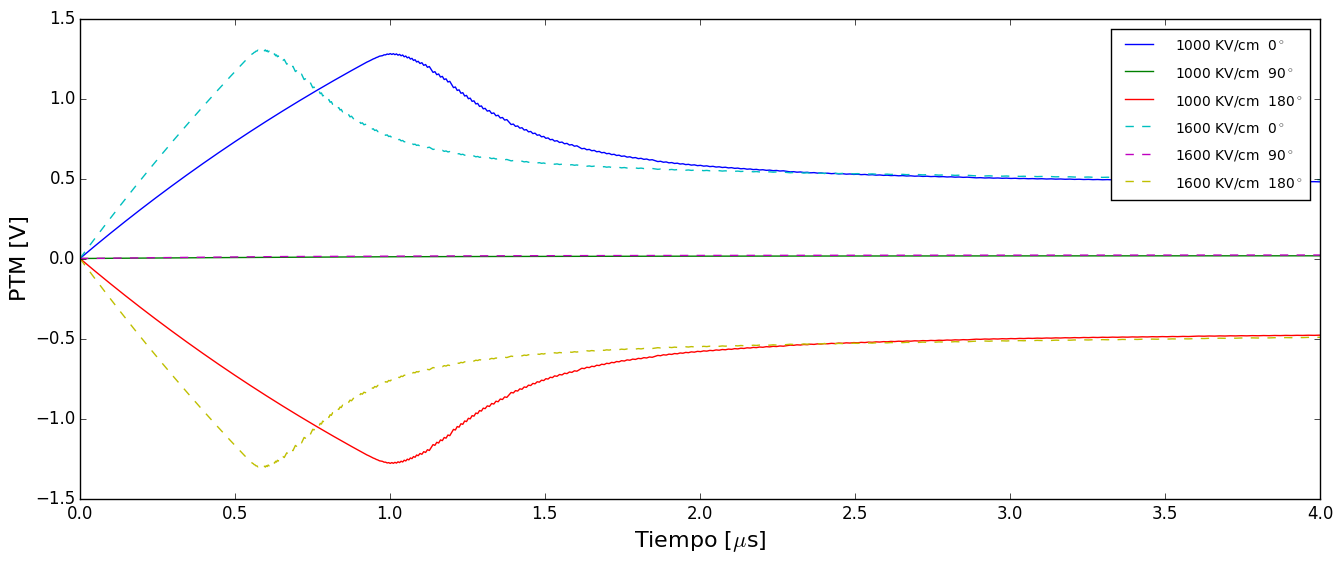
\includegraphics[width=\linewidth]{poros/itv-time}
	\caption{PTM en función del tiempo en distintos ángulos polares para dos potenciales aplicados diferentes}
	\label{fig:itv-time}
\end{figure}

%Se puede observar en la figura \ref{fig:itv-time} el potencial transmembrana en función del tiempo al comienzo del pulso para diferente ángulos polares $\theta$. Las cuatro figuras corresponden a cuatro pulsos de diferente potencial eléctrico aplicado sobre la misma célula. En el primer caso el potencial eléctrico es muy chico y por lo tanto no se alcanzaron a crear poros. En los otros casos el potencial sí es lo suficientemente alto como para crear poros. Se observa en estos casos que el PTM se incrementa durante los primeros instantes hasta alcanzar un pico de tensión a partir del cual comienza a disminuir hasta alcanzar un valor de equilibrio. La subida paulatina de tensión durante los primeros instantes del pulso se debe a la capacitancia de la célula, mientras que la caída en los instantes posteriores se debe a la aparición de poros, que disminuyen la conductividad de la membrana, disminuyendo de esta manera la caída de tensión entre el interior y exterior de la célula. 

%Se nota en todos los casos que las regiones de la membrana cercanas a los polos (con ángulos cercanos a 0º o 180º) obtienen en los primeros instantes los valores absolutos de PTM más altos, mientras que las regiones cercanas al ecuador (ángulo polar cercano a 90º) tienen un PTM prácticamente nulo.

Se puede observar en la figura \ref{fig:itv-time} el potencial transmembrana en función del tiempo al comienzo del pulso para diferentes ángulos polares $\theta$, con dos campos eléctricos diferentes. El PTM se incrementa durante los primeros instantes hasta alcanzar un pico de tensión a partir del cual comienza a disminuir hasta alcanzar un valor de equilibrio. La subida paulatina de tensión durante los primeros instantes del pulso se debe a la capacitancia de la célula, mientras que la caída en los instantes posteriores se debe a la aparición de poros, que disminuyen la conductividad de la membrana, disminuyendo de esta manera la caída de tensión entre el interior y exterior de la célula. Se nota que el PTM obtenido depende notablemente del ángulo polar: en la región polar cercana al electrodo positivo el PTM es positivo y alcanza valores altos, mientras que en el polo cercano al cátodo el potencial es negativo y en el ecuador es cercano a cero. Es llamativo que los valores de campo eléctrico aplicado no influyen en el valor de pico de PTM obtenido, pero si en el tiempo en que éste se alcanza; al aumentar el campo de 1000\vcm a 1600\vcm se acelera el proceso de subida y bajada de PTM hasta alcanzar un equilibrio, pero no se logran aumentar los potenciales obtenidos.


%aca poner gráficos de PTM vs ángulo para diff tiempos. estaría bueno poner una sola curva por gráfico y gráficos más chicos. podrian ser todos de un solo potencial en vez de diferentes tensiones

\dobleimagengrande{poros/120kvm/tita}{tita120}{PTM en función del ángulo polar\\ con $E = 1200\,\vcm$}{poros/160kvm/tita}{tita160}{PTM en función del ángulo polar\\ con $E = 1600\,\vcm$}

En las figuras \ref{fig:tita120} y \ref{fig:tita160} se graficaron los potenciales transmembrana en función del ángulo polar para diferentes instantes de tiempo con pulsos de potenciales diferentes en los dos gráficos. Se observa en los primeros instantes que el PTM obtenido es similar al obtenido en el capítulo anterior y al que se puede estimar con la fórmula cerrada \ref{eq:cos}. Esto se debe a que la población de poros es nula o muy pequeña como para afectar aún la conductividad de la membrana. Sin embargo en los instantes posteriores la aparición de poros disminuye notablemente la conductividad de la membrana en las regiones cercanas a los polos, bajando así la diferencia de potencial. En instantes posteriores se observa el mismo fenómeno con regiones más lejanas a los poros, alejándose más el PTM obtenido del que se puede calcular con la fórmula cerrada \ref{eq:cos}.\\

%%%%

Se estudió también el efecto de aplicar una señal de varios pulsos en lugar uno solo. En la figura \ref{fig:poros-tiempo} se graficó la cantidad de poros en función del tiempo para 4 pulsos de 5\ms de \ontime{} y 5\ms de \offtime{} con varios potenciales diferentes. Se puede ver que la cantidad de poros crece únicamente al principio de cada pulso, y se mantiene casi constante durante el resto del pulso, disminuyendo muy levemente durante el tiempo de apagado. Por cada pulso nuevo se crean poros nuevos, aunque la cantidad de poros nuevos disminuye con cada pulso consecutivo. Se puede ver también que el efecto del campo eléctrico sobre la densidad es enorme, obteniéndose poblaciones de casi el doble de poros para al aumentar el potencial aplicado de 1200\vcm a 1600\vcm. El valor 500\vcm como valor mínimo necesario para obtener una cantidad considerable de poros, mientras que para 400\vcm y otros valores menores la densidad es despreciable, es decir casi no se produce electroporación. 

En la figura \ref{fig:radios-tiempo} se graficó el promedio de los radios de los poros en función del tiempo. Se nota que los radios altos se obtienen por un instante muy corto de tiempo al principio de cada pulso, y que rápidamente se achican llegando a un valor de equilibrio en aproximadamente la mitad del tiempo del \ontime. Cuando el pulso se apaga, los radios se hacen rápidamente mínimos, y se mantienen en un valor muy chico hasta el inicio del próximo pulso. A diferencia de la cantidad de poros, el radio promedio disminuye al aumentar el potencial eléctrico. Esto puede deberse a que un mayor campo eléctrico produce muchos poros de radio mínimo, afectando el promedio de manera negativa. En cada pulso consecutivo parecen aumentar ligeramente los radios obtenidos, notándose la mayor diferencia entre los radios del primer y el segundo pulso. 

En las figuras \ref{fig:pulso1} a \ref{fig:pulso4} se observan las distribuciones de radios de poros para 1600\vcm al instante de 100\usec luego del comienzo de cada pulso. Las diferencias entre radios se observan sobre todo entre el primer y segundo pulso, mientras que los siguientes parecen tener distribuciones muy similares. La mayor concentración se encuentra siempre en los radios muy pequeños (de aproximadamente 1 \si{\nano\metre}), que afectan poco al proceso de permeabilización de la membrana.



\imagensola{poros/poros-tiempo}{poros-tiempo}{Cantidad de poros en función del tiempo para cuatro pulsos}{}
\imagensola{poros/radios-tiempo}{radios-tiempo}{Radio promedio de los poros en función del tiempo para cuatro pulsos}{}



%En las figuras \ref{pulso1} a \ref{pulso4} se observan las distribuciones de radios de poros para cuatro pulsos consecutivos. Los pulsos son de 160\kvcm con 5\ms de \ontime{} y 5\ms de \offtime{} y los histogramas corresponden al instante de 100\usec luego de comenzado cada pulso. \todo[inline]{escribir más después de poner cant poros vs tiempo}

%\dobleimagengrande{poros/160kvm/pulso1}{pulso1}{Primer pulso}{poros/160kvm/pulso2}{pulso2}{Segundo pulso}
%\dobleimagengrande{poros/160kvm/pulso3}{pulso3}{Tercer pulso}{poros/160kvm/pulso4}{pulso4}{Cuarto pulso}

\begin{figure} [ht!]
\makebox[\textwidth][c] {
	\centering
	\begin{minipage}{.43\paperwidth}
		\centering
		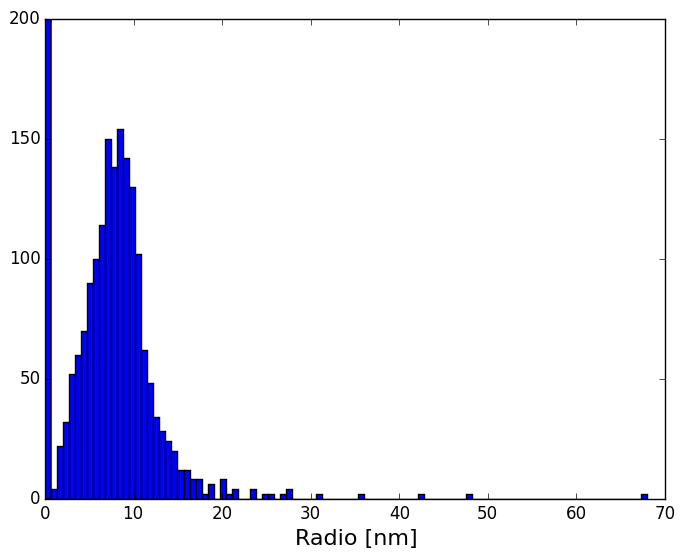
\includegraphics[width=1\linewidth]{poros/160kvm/pulso1}
		\captionof{figure}{Primer pulso}
		\label{fig:pulso1}
	\end{minipage}%
	\begin{minipage}{.43\paperwidth}
		\centering
		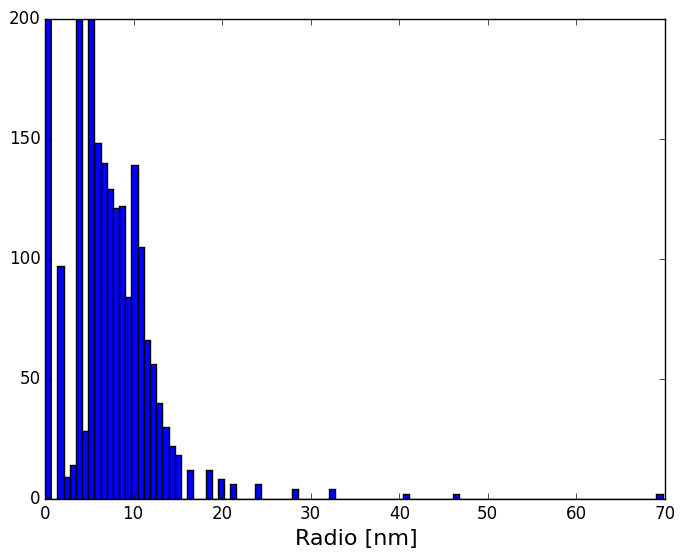
\includegraphics[width=1\linewidth]{poros/160kvm/pulso2}
		\captionof{figure}{Segundo pulso}
		\label{fig:pulso2}
	\end{minipage}
}
\end{figure}

\begin{figure} [ht!]
\makebox[\textwidth][c] {
	\centering
	\begin{minipage}{.43\paperwidth}
		\centering
		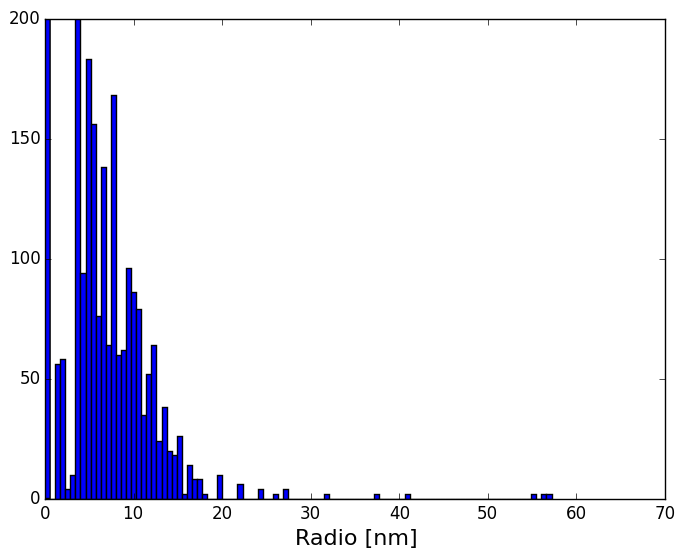
\includegraphics[width=1\linewidth]{poros/160kvm/pulso3}
		\captionof{figure}{Tercer pulso}
		\label{fig:pulso3}
	\end{minipage}%
	\begin{minipage}{.43\paperwidth}
		\centering
		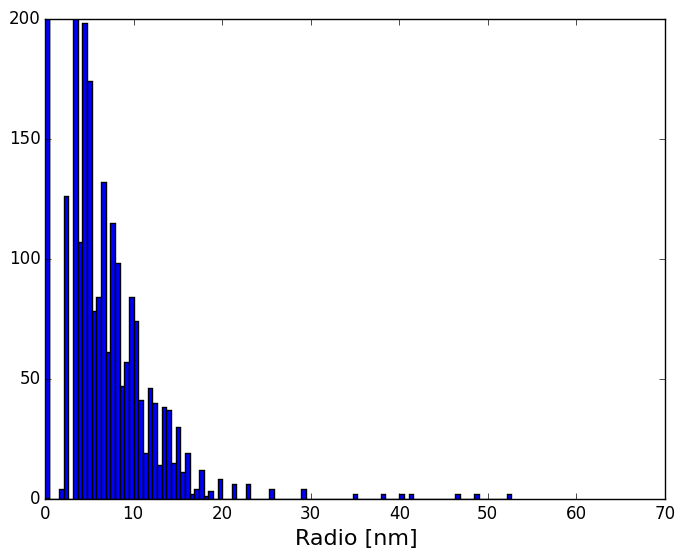
\includegraphics[width=1\linewidth]{poros/160kvm/pulso4}
		\captionof{figure}{Cuarto pulso}
		\label{fig:pulso4}
	\end{minipage}
}
\end{figure}

%TODO conclusiones generales
%TODO mencionar potencial mínimo necesario para electroporación. podría ir tmb un gráfico de itv en tiempo con voltaje bajo sin electroporación
%TODO mencionar que la formula cerrada de itv no sirve


\chapter{Transporte de Especies}
% CAP 5 Transporte. idem (solo transporte, sin poros)

En este capítulo se analiza la concentración y movimiento de cuatro especies iónicas: el hidrógeno (\h), el hidróxido (\oh), el sodio (\na) y cloruro (\cl) en el dominio producto del campo eléctrico aplicado. Para ello se realizan simulaciones en las que se aplican pulsos eléctricos a las mallas generadas anteriormente y se analiza el transporte de las cuatro especies producto del gradiente de concentración y del campo eléctrico según la ley de Nernst-Planck. Se ignora en este capítulo la creación de poros en la membrana celular.\\

\section{Implementación}

%Como las concentraciones de las cuatro especies son independientes entre sí, se hace uso de la interfaz OpenMP para realizar llenar las matrices y resolver los sistemas en cada iteración. 

\section{Resultados}
Para esto hace falta correr sin poros y escribir algo.

\chapter{Modelo Acoplado}
% CAP 6 Todo acoplado. Resultados. poner snapshots de valores 1-9

En este capítulo se realizan simulaciones de todos los fenómenos físicos simulados en los capítulos anteriores juntos, es decir el potencial eléctrico, la creación de poros en la membrana y la posterior variación en el radio de los mimos, las variaciones en la conductividad y difusión de la membrana producto de la aparición de poros y el transporte de especies iónicas en el dominio. Además se estudió el efecto de aplicar varios pulsos consecutivos a través de los electrodos, en lugar de un único pulso.

\section{Implementación}
Para realizar la simulación completa se creó un ciclo principal que realiza llamados a las diferentes rutinas implementadas en los capítulos anteriores.\\

Para acelerar los tiempos de ejecución se usaron intervalos temporales diferentes para los distintos fenómenos físicos simulados. Para el cálculo de la densidad de poros en la membrana celular y sus radios se utilizó un intervalo temporal muy pequeño, ya que se notó que al aumentarlo se producen errores de discretización muy grandes que producen la divergencia del sistema. Para el cálculo de los potenciales eléctricos en el dominio, en cambio, alcanzó un intervalo temporal mucho mayor, y se notó que reducirlo no impacta en los resultados. Por último para el cálculo de las concentraciones de las especies iónicas se necesitaron intervalos temporales aún mayores. Concretamente se usaron intervalos de 1 \si{\nano\second} para las ecuaciones de poros, 20 \si{\nano\second} para el transporte de especies y un intervalo variable de entre 1 \si{\nano\second} y 2 \si{\micro\second} para el cálculo del potencial eléctrico. Este último intervalo es variable dado que los primeros instantes de cada pulso eléctrico es el que tiene mayores variaciones en los potenciales producto de la repentina permeabilización de la membrana, como puede verse en el capítulo 4. Esto hace que se necesite una actualización constante de los valores de potencial en los nodos, sobre todos los cercanos a la membrana celular. Sin embargo pasados los primeros microsegundos del pulso el sistema se estabiliza y la permeabilización y valores de PTM se mantienen con pocos cambios lo que hace innecesario un cálculo constante de los potenciales. Por esta razón se optó por un intervalo muy pequeño al comenzar un pulso y se incrementa de manera exponencial.\\

%TODO revisar los valores de los intervalos!! revisar si transporte efectivamente mayor que poisson
%TODO está bien decir delta t exponencial? aumenta como un capacitor

%TODO on time, off time. mencionar que se reinicia el delta_t

%TODO mencionar truco numérico temperatura

\section{Resultados}

Se presentan a continuación las concentraciones en el dominio de las diferentes especies iónicas estudiadas para diferentes instantes de tiempo. Los resultados corresponden a simulaciones de una célula de ??? bajo ? pulsos eléctricos con una diferencia potencial de ??? y una duración de ??? encendidos y ??? apagados cada uno.\\

Tener primero resultados para poder escribir.

\subsection*{\h}

Acá poner snapshots de pH \\

\subsection*{\oh}

\subsection*{\na}

\subsection*{\cl}


\chapter{Conclusiones}
% CAP 7 conclusiones

\backmatter
\bibliography{tesis}

\begin{thebibliography}{99}

%TODO agregar títulos a los que les falta!!
%TODO poner nombres en lugar de iniciales

\bibitem{c1}
	Colombo L., González G., Marshall G., Molina F., Soba A., Suárez C., Turjanski P.
	Bioelectrochemistry 71,
	2007

\bibitem{c2}
	Nilsson E, von Euler H, Berendson J, Thorne A, Wersall P, Naslund I, Lagerstedt A, Narfstrom K, Olsson J
	Bioelectrochemistry 51,
	2000

\bibitem{c3}
	Netti PA, Berk DA, Swartz MA, Grodzinsky AJ, Jain RK
	Cancer Research 60,
	2000

\bibitem{c4}
	Matías Daniel Marino, Dr. Pablo Turjanski, Dr. Nahuel Olaiz
	\emph{Electroporación en el tratamiento de tumores: modelos teóricos y experimentales}
	2013

\bibitem{c5}
	G. Puchiar, T. Kotnik, B. Valic and D. Miklavcic
	\emph{FALTA EL NOMBRE!!!}
	Annals of Biomedical Engineering
	Volume 34, 4, 2006

\bibitem{c6-fodava}	
	Qiong Zheng, Duan Chen, Guo-Wei Wei
	\emph{FALTA EL NOMBRE!!!}
	Journal of Computational Physics,	
	Volume 230, 13, 2011

\bibitem{c7-krass07}	
	Wanda Krassowska, Petar D. Filev,
	\emph{FALTA EL NOMBRE!!!}
	Biophysical Journal, Volume 92, Issue 2, 2007

\bibitem{c8}
	Jianbo Li, Hao Lin
	\emph{Numerical simulation of molecular uptake via electroporation}
	Bioelectrochemistry 82, 10–21, 2011 

\bibitem{c9-fem-electro}
	Stanley Humphries
	\emph{Finite-element Methods for Electromagnetics}
	2010

\bibitem{c10}
	O.C. Zienkiewicz, R.L. Taylor
	\emph{The Finite Element Method Volume I: The Basis}
	Butterworth-Heinemann, 5th edition, 2000

\bibitem{c11}
	\emph{Automesh 2D}
	\texttt{http://www.automesh2d.com/}

\bibitem{c12}
	Geoffrey M. Cooper, Robert E. Hausman
	\emph{La Célula}
	2$^{\circ}$ edición, 
	Marbán

\bibitem{c13}	
	P.H. Mott, J.R. Dorgan, C.M. Roland 
	\emph{The bulk modulus and Poisson's ratio of incompressible materials} 
	Journal of Sound and Vibration 312, 572–575, 2008
	
\bibitem{c14}
	John David Jackson
	\emph{Classical Electrodynamics}
	3$^{\circ}$ edición,
	John Wiley \& Sons Inc.,
	1999

\bibitem{c15}	
	Antonio Nives
	\emph{Métodos numéricos aplicados a la ingeniería}
	Grupo editorial Patria,
	2007

\bibitem{c16}
	\emph{Paraview}
	\texttt{www.paraview.org}
	Sandia National Laboratory, Kitware Inc, Los Alamos National Laboratory

\bibitem{matplotlib}
	\emph{matplotlib}
	\texttt{http://matplotlib.org/}
	

%\bibitem{krass}
%	Wanda Krassowska and Petar D. Filev
%	\emph{Modeling Electroporation in a Single Cell}
%	Biophysical Journal
%	Volume 92, Issue 2, 15 January 2007, Pages 404–417

\bibitem{tsong}
	Tsong, T. Y.
	\emph{Electroporation of cell membranes}
	Biophys. J. 60:297–306, 1991

\bibitem{krass-viejo}
	Katherine A. DeBruin, Wanda Krassowska, 
	\emph{Modeling Electroporation in a Single Cell. I. Effects of Field Strength and
Rest Potential}
	Biophysical Journal, Volume 77, 1999
	
\bibitem{eigen}
	\emph{Eigen}
	\texttt{http://eigen.tuxfamily.org/}
	
\bibitem{burden}
	Richard L. Burden, J. Douglas Feires
	\emph{Análisis numérico}
	Séptima edición, I.T.P. Latin America, 2001

\bibitem{yousef}
	Yousef Saad
	\emph{Iterative Methods for Sparse Linear Systems}
	Seguna edición, Society for Industrial and Applied Mathematics, 2003
	
\end{thebibliography}


\end{document}
